\chapter{深度学习概念与现有视频目标跟踪算法理论}
\section{深度学习基础概念}
深度学习(Deep Lrarning)是以深度神经网络为模型结构的机器学习算法\supercite{deng2014deep}.机器学习(Mechine Learning)通常指一些依靠计算机确定模型的建模方法.目前大多数机器学习算法还无法完全自行实现学习,通常只能在人为规定的模型下,针对某个小问题对特定的数据建模.
\par
机器学习,模式识别等学科最终试图解决的问题通常是建立模型,解决问题.如目标跟踪即可描述为输入是视频,输出是轨迹的问题.神经网络(Neural Network, NN)由于其优秀的非线性拟合能力,成为如今机器学习最常用的模型结构之一.
\subsection{神经网络}
神经网络最初的灵感一部分来源于仿生学\supercite{mcculloch1943logical}\supercite{farley1954simulation},这也是神经网络的灵魂思想.
\par
相比于k-NN,SVM(支持向量机),线性回归(linear regression)等传统机器学习算法,神经网络主要依靠激活函数(activation function)得到非线性效果.为了避免梯度消失的问题,近期的研究与应用中最常用的激活函数是ReLU激活函数\supercite{krizhevsky2012imagenet}.不同的激活函数会有不同效果\supercite{karlik2011performance}.
\par
而相比与各种树模型,神经网络又有更好的泛华能力.
\par
最简单的神经网络结构是全连接的(Fully Connected, 有时简称FC)神经网络, 该结构又称多层感知机(Multi Layer Perceptron, 简称MLP).多层感知机由多个层$l_1,l_2,...l_n$依次排列组成.每个层由许多神经元组成,某以层上的每个神经元将接受上一层所有神经元为输入,并向下一层的所有神经元输出.以ReLU为激活函数,位第k层的第m个神经元的输出为$output_{k,m}=ReLU(\sum_{i} (output_{k-1,i}*w_{k,m,i})+b_{k,m})$,其中$w_{k}$和$b_{k}$是属于第k层的变量,通常经过训练得出.
\par
全连接神经网络的连接较多,参数也会更多,即所有参数组成的参数向量很稀疏,不利于训练.通常只在最终将多维的状态量收敛成低维结果时使用.在前期对高维的数据的处理过程中,常常会对神经网络的结构进行一定简化,减少连接以利于训练.常用的减少连接方式有卷积神经网络和循环神经网络等.
\par
\subsubsection{卷积神经网络}
\par
\begin{figure}[htbp!]
    \centering
    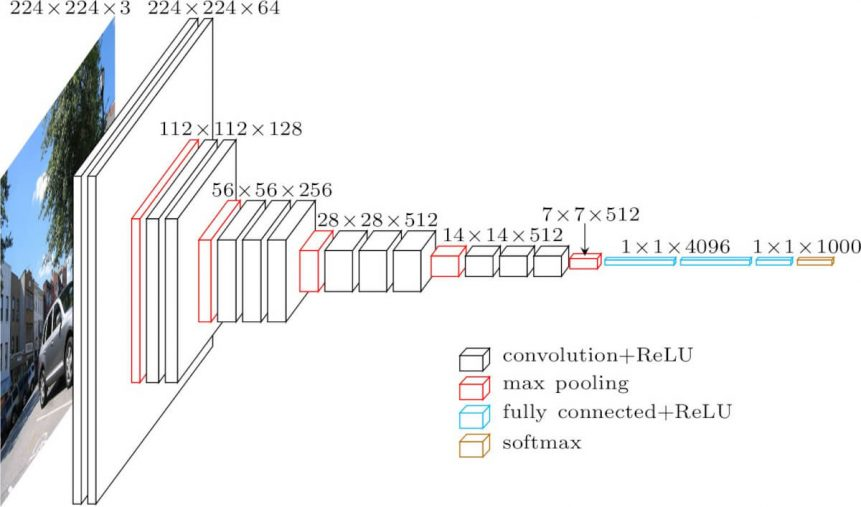
\includegraphics[width = 1.\textwidth]{chap/img/vgg16-neural-network.jpg}
    \caption{
        用于图像分类的VGG16\supercite{simonyan2014very}卷积神经网络结构图.图片来自 \url{https://neurohive.io/en/popular-networks/vgg16/}
        }\label{fig:vgg16_architecture}
\end{figure}
\par
卷积神经网络(Convolutional Neural Network, CNN)是一种为图像处理设计的神经网络结构.同全连接神经网络一样,卷积神经网络也分为很多层,每一层只与前一层和后一层连接.不同的是,每层的一个神经元只连接前一层与后一层的少部分神经元.通常,CNN的每一层可以用一个多波段图像表示,连接只建立在前一层与后一层位置接近的像素上.类似图像处理中的模板滤波方法.常用的CNN的模板大小是$3*3$,有时也可以是$5*5$,$7*7$等大小.每一层的所有神经元公用一个模版,模版上所有的参数都是训练得到的变量.卷积神经网络同样要在每层上加入激活函数,常用ReLU激活函数.
\par
完整的卷积神经网络通常会在卷积层中穿插池化(Pooling)层以收敛数据维度.池化层可以将卷积层图片大小减小.常用的配合ReLU激活函数的池化层如最大值池化(Max Polling)方法.以$2*2$为池的大小的池化层的输出为输入层大小的一半,每个像元为对应位置的4个像元的最大值.
\par
以图像分类问题为例,该问题需要输出一个较低维度的结果,即图像属于是每个类别的概率,可以用一个向量表示.用于图像分类的神经网络通常使用CNN层与最大值池化层交替减小图像大小,最终用全连接层得到分类结果.如图\ref{fig:vgg16_architecture}所示的VGG16\supercite{simonyan2014very}卷积神经网络即是这样一个图像分类算法.
\begin{figure}[htbp!]
    \centering
    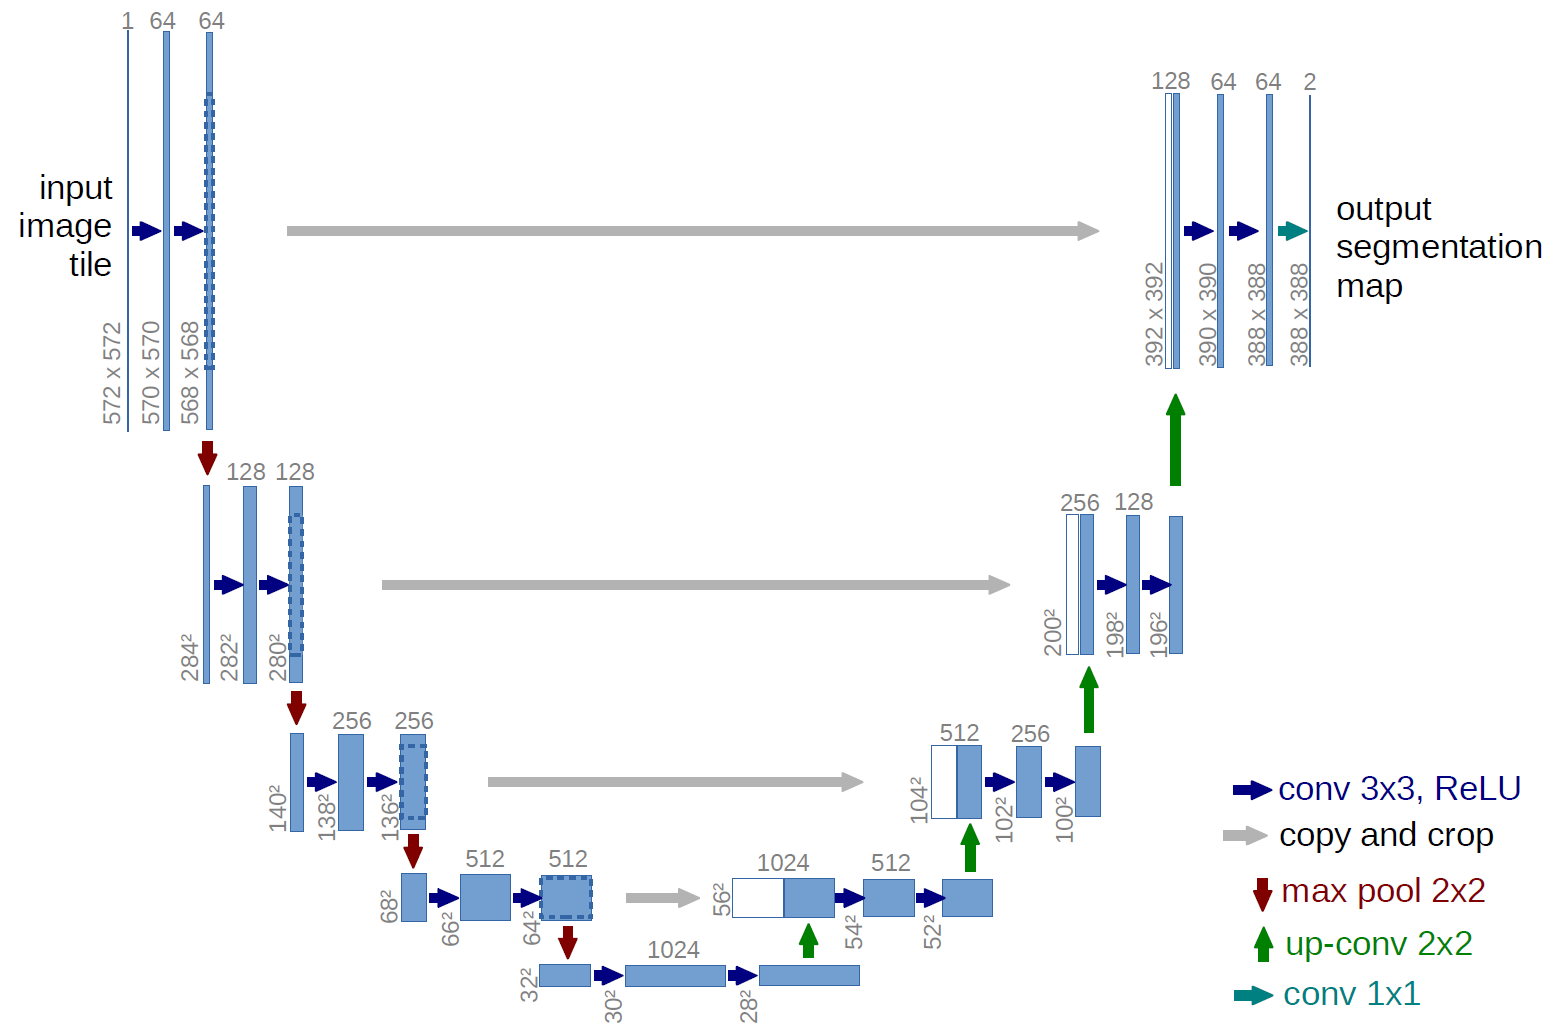
\includegraphics[width = 1.\textwidth]{chap/img/u-net-architecture.png}
    \caption{
        用于图像分割的U-Net\supercite{ronneberger2015u}卷积神经网络结构图.
        }\label{fig:unet_architecture}
\end{figure}
\par
不同于图像分类,图像分割等像素级图像处理问题需要得到更高维的结果,且得到的结果需要有一定的空间特性.如图\ref{fig:unet_architecture}的U-Net是一种常用的处理分割等像素级别问题的卷积神经网络.该网络有加密和解码两个步骤,加密阶段图像经过多次卷积和池化变小,蕴含的信息更宏观;而解码阶段图像经过反卷积(Deconvolution)操作再次放大,得到与原图大小相似的结果.类似的还有SegNet\supercite{badrinarayanan2017segnet}卷积神经网络等.
\par
U-Net的网络结构为像素级别处理提供了思想基础.
\par

\subsubsection{循环神经网络}
RNN(循环神经网络, 又称递归神经网络, Recurrent Neural Network)是深度学习处理序列问题,尤其是时间序列数据时的重要方法.上文中介绍了全连接和卷积神经网络,这两种结构的神经网络接受的输入都是由网络结构事先确定的.如针对图像处理问题,通常的做法是将图片采样,拉伸至CNN的输入要求再进行处理.当进行时间序列分析时,这样的结构只能接受定长的时间序列数据.但实际上大多数时间序列数据是变长的.
\par
RNN能很好解决这个问题.RNN可以将参数相同的某个神经单元重复使用多次以处理.通常情况下\footnote{这里介绍的RNN全是单向RNN,且对时间序列处理的先后顺序为时间流逝的顺序},RNN
\subsubsection{反向传播求梯度法}

\section{视频跟踪算法}
受限于目前计算机的计算能力,我们不能随意增大算法的规模,因为在大多数情况下不能实时进行目标跟踪的方法是没有意义的.因此视频目标跟踪算法必须要节约计算资源.因而算法的设计就显得格外重要.
\subsection{运动模型}
运动模型是用于描述目标的运动的模型.本文中运动模型蕴含的信息包括目标的运动与目标的形态变化.
\par
\begin{figure}[htbp!]
    \centering
    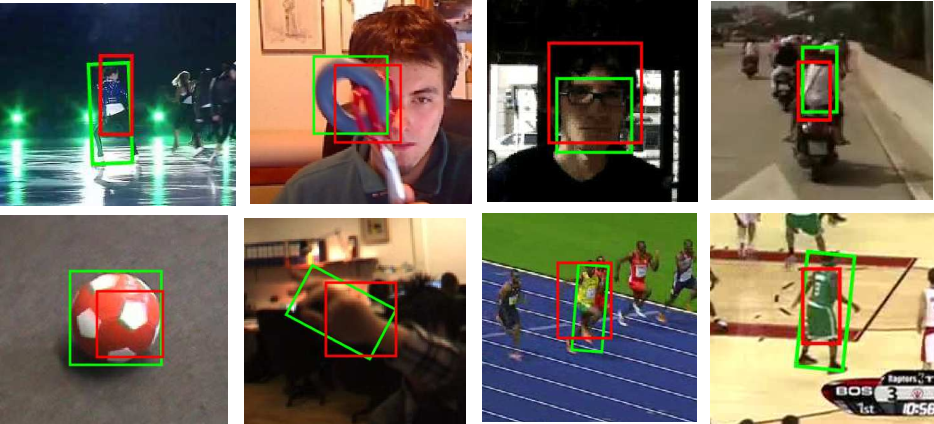
\includegraphics[width = 1.\textwidth]{chap/img/overlap_examples.pdf}
    \caption{用于描述跟踪目标的外包矩形.红色:限定竖直的的外包矩形;绿色:不限定竖直的外包矩形.原图片为VOT竞赛中描述标记与目标的插图\supercite{VOT_TPAMI}}\label{fig:bunding_boxes}
\end{figure}
\par
常见的矩形框视频目标跟踪算法考虑会考虑目标的最小外包矩形(Bounding Box)和位置(Location).最小外包矩形的方向有时是限定为竖直的,即矩形的上下边平行于图像的上下边,左右边同理;有时不限定,可以是任何方向.限定竖直与不限定竖直的矩形表示法如图\ref{fig:bunding_boxes}所示.位置一般用矩形的中心表示.
\par
像素级跟踪算法的运动模型需要表达的信息与矩形框跟踪算法类似

\chapter{基于CNN和RNN的素级别跟踪算法}
本章是本文的重点,将详细介绍本研究的理论创新.
\par
本研究提出一种结合现有的像素级别处理技术和现有的矩形级视频目标跟踪技术的像素级别目标跟踪算法,具体算法结构,实现细节,训练等将在本章重点介绍.
\section{算法结构与核心思想}
本文所实现的算法将首先基于用于实现静态图像分割的U-Net\supercite{ronneberger2015u}的多级降级-升级卷机神经网络结构.但将在这个多级网络结构中加入Conv-LSTM结构.
\par
类似与U-Net的结构,本文的卷机网络部分也将有多个降级和升级结构;每个降级结构包括几个卷积层,使用池化结构进行降级;每个升级部分采用升卷积进行升级处理.在降级过程中,图片数据的尺寸大小会衰减,同时等比例增加其波段范围.对于3层的结构,最小级的波段将有128个.这个多级结构的设计理念是为了处理多尺度问题;浅层的级别能很好的处理细节问题,但对宏观的把控会较弱,具体表现为可能会出现噪声点;深层的结构对宏观把控好,但对边界处理较弱.升级结构能将浅层处理得到的边界信息与深层处理得到的宏观信息相结合,得到一个更好的结果.
\par
在时间尺度,本研究的算法将主要采用LSTM算法解决问题.具体的,LSTM单元将被加入到各个层级当中.LSTM在各种跟踪算法中有广泛应用,但大多数算法仅仅将其作为对最后结果的处理手段.本研究的算法将把LSTM作为所有的中间状态记录单元.
\par
与纽约大学2017年实现的Conv-LSTM结构的跟踪算法不同的是,本文所采用的多级神经网络将把Conv-LSTM加入各个卷机层级;而与U-Net,SegNet等多级分割算法不同的是,本文将在整个结构中多处穿插LSTM以得到一个时间连续的结果.
\section{基于CNN和RNN的像素级别跟踪模型在空间维度的处理}
\subsection{CNN的原理}
\subsection{多尺度思想的引入}
\section{基于CNN和RNN的像素级别跟踪模型在时间维度的处理}
\subsection{RNN的原理}
\subsection{跟踪状态}
\subsection{跟踪系统初始化}


% TODO 删除下边的,移到第三章
\section{模型训练}
本章前文中提出的模型结构是一个深度神经网络,它需要配合参数才可以运行.参数的获取过程称为模型训练.

\subsection{机器学习算法}

\subsection{模型训练原理}
模型训练(Train)是机器学习中获取参数的过程.典型的模型训练方法是梯度下降法.本研究的模型也将用梯度下降法求取参数.
\subsubsection{梯度下降法}

\subsubsection{求梯度:反向传播算法}
反向传播是常用的深度神经网络求梯度的方法.